\documentclass{bmstu}

\bibliography{biblio}

\begin{document}

\makecourseworktitle
	{Информатика и системы управления}
	{Программное обеспечение ЭВМ и информационные технологии}
	{Визуализация модели цветка}
	{Жаворонкова~А.~А./ИУ7-56Б}
	{Куров~А.~В.}
	{}

\setcounter{page}{3}
\maketableofcontents

%\begin{definitions}
	\definition{}{}
\end{definitions}
%\begin{abbreviations}
	\definition{}{}
\end{abbreviations}

\chapter*{ВВЕДЕНИЕ}
\addcontentsline{toc}{chapter}{ВВЕДЕНИЕ}

Целью данной работы является разработка программного обеспечения для создания реалистичного изображения цветка. Программа должна предоставлять возможность изменения положения камеры и источника освещения.

Для достижения поставленной цели требуется решить следующие задачи:
\begin{itemize}[label=---]
	\item выделить объекты сцены и выбрать модель их представления;
	\item проанализировать алгоритмы визуализации трехмерной сцены, при необходимости рассмотреть модификации, обосновать выбор конкретного алгоритма;
	
	\item  реализовать выбранные алгоритмы;
	
	\item спроектировать архитектуру и графический интерфейс программы;
	\item реализовать программное обеспечение для визуализации модели цветка;
	\item исследовать зависимость скорости генерации кадра от шага полигональной сетки.
\end{itemize}
\chapter{Аналитический раздел}

\section{Формализация объектов синтезируемой сцены}

Сцена состоит из следующих объектов:
\begin{enumerate}
	\item Ограничивающая плоскость --- расположена параллельно плоскости OXZ;
	\item Цветок --- расположен на ограничивающей плоскости. В нем можно выделить следующие составляющие:
	\begin{enumerate}[label*=\arabic*.]
		\item Стеблевая часть:
		\begin{enumerate}[label=\alph*)]
			\item Цветоножка --- длинный изогнутый цилиндр, описываемый следующими уравнениями:
			\begin{equation*}
				\begin{cases}
					x = 0.6\cos t + \frac{1}{5}\sin z,\\
					y = 0.6\sin t,\\
					z = z.
				\end{cases}
			\end{equation*}
			где $t \in [0;2\pi), z \in [0;20]$. 
			Здесь $z$ определяет высоту стебля. Выбор интервала основывался на размерах остальных частей цветка.
			
			\item Цветоложе --- часть эллипсоида, задаваемая уравнением:
			\begin{equation*}
				z = \frac{(x - \frac{1}{4})^2}{2} + \frac{y^2}{2}
			\end{equation*}
			при $x \in [-2.25; 2.75], y \in [-2.5;2.5]$.
			Интервалы для $x$ и $y$ были выбраны таким образом, чтобы часть эллипсоида имела характерные для цветоложа углубления.
			
			\item Лист --- поверхность, ограниченная парой кривых, описываемых следующими уравнениями:
			\begin{equation*}
				\begin{cases}
					x = t,\\
					y = \frac{1}{3}t^2,\\
					z = \frac{2}{t+1} + 3t.
				\end{cases}
			\end{equation*}
			где $t \in [0;5.2]$.
			
			Вторая кривая получается в результате поворота первой кривой на угол $\phi = \frac{-\pi}{3}$. Полученные уравнения, задающие вторую кривую:
			\begin{equation*}
				\begin{cases}
					x = t\cos\frac{-\pi}{3}-\frac{1}{3}t^2\sin\frac{-\pi}{3},\\
					y = t\sin\frac{-\pi}{3}+\frac{1}{3}t^2\cos\frac{-\pi}{3},\\
					z = \frac{-2}{t-1}-3t.
				\end{cases}
			\end{equation*}
			где $t \in [-5.2;0]$.
			
			Описанные выше кривые пересекаются в точках:
			$$ A(0;0;2), B(3\sqrt{3}; 9; \frac{2}{3\sqrt{3}} +9\sqrt{3}) $$
			
		\end{enumerate}
		\item Листовая часть --- совокупность поверхностей, образующих непосредственно лепестки цветка. Один лепесток описывается системой:
		\begin{equation*}
		\begin{cases}
			z = \frac{1}{2}x^2+y\\
			x^2+\frac{1}{5}y^2 \leq 3
		\end{cases}
		\end{equation*}
	\end{enumerate}
	\item Источник освещения --- начальное положение источника указывается по умолчанию, но пользователь может его изменить;
	\item Камера --- начальное положение источника указывается по умолчанию, но пользователь может его изменить.
\end{enumerate}

\section{Выбор способа определения моделей}

Модели могут задаваться в следующих формах \cite{models}:
\begin{itemize}[label=---]
	\item \textbf{Каркасная модель.} В данной модели задается информация о вершинах и ребрах объекта. Это одна из простейших форм задания модели. Основная проблема отображения объектов с помощью каркасной модели заключается в том, что модель не всегда однозначно передает представление о форме объекта.
	\item \textbf{Поверхностная модель.} Данный тип модели часто используется в компьютерной графике. Поверхность может описываться аналитически, либо задаваться другим способом. Недостатком поверхностной модели является отсутствие информации о том, с какой стороны поверхности находится материал.
	\item \textbf{Твердотельная модель.} Данная форма задания модели отличается от поверхностной формы тем, что в объемных моделях к информации о поверхностях добавляется информация о том, с какой стороны расположен материал. Это можно сделать путем указания направления внутренней нормали.
\end{itemize}

При рассмотрении объектов было сказано, что они представляют собой поверхности. Поэтому для решения поставленной задачи была выбрана поверхностная форма модели.

\section{Выбор алгоритма удаления невидимых ребер и поверхностей}

Алгоритмы удаления невидимых линий и поверхностей служат для определения поверхностей или объемов, которые видимы или невидимы для наблюдателя, находящегося в заданной точке пространства. Решать поставленную задачу удаления можно как в объектном пространстве (в мировой системе координат), так и в пространстве изображения (в экранных координатах).

Рассмотрим алгоритмы для удаления невидимых ребер и поверхностей.

\subsection{Алгоритм Робертса}

Алгоритм работает в объектном пространстве. Требуется, чтобы все изображаемые тела были выпуклыми. 

Алгоритм работает в 3 этапа: подготовка исходных данных, удаление ребер, экранируемых самим телом, удаление ребер, экранируемых другими телами.

\textbf{Этап 1. Подготовка исходных данных.}

Необходимо сформировать матрицы тел, которые будут представлять выпуклые твердые тела. В такой матрице каждый столбец содержит коэффициенты одной плоскости. При этом точки, лежащие внутри тела, дают положительное скалярное произведение с каждым столбцом матрицы.

\textbf{Этап 2. Удаление ребер, экранируемых самим телом.}

На данном этапе используется вектор направления взгляда: 
$$ E = [0; 0; -1; 0]$$
При умножении вектора E на матрицу тела отрицательные компоненты полученного вектора будут соответствовать задним граням. Если объект на сцене один, то работа алгоритма завершается на данном этапе.

\textbf{Этап 3. Удаление ребер, экранируемых другими телами.}

Необходимо провести луч из произвольной точки анализируемого отрезка в точку наблюдения. Если луч проходит через тело, то точка невидима, а луч расположен с положительной стороны от каждой грани тела.

\textbf{Преимущества \cite{rojers}:}
\begin{itemize}[label=---]
	\item Точность вычислений благодаря тому, что алгоритм работает в объектном пространстве;
	\item Использование математически простых и точных методов.
\end{itemize}

\textbf{Недостатки \cite{rojers}:}
\begin{itemize}[label=---]
	\item Возможность работать только с выпуклыми объектами;
	\item Сложность алгоритма $O(n^2)$, где $n$ --- количество объектов сцены.
\end{itemize}

\subsection{Алгоритм, использующий z-буфер}

Алгоритм работает в пространстве изображения. Основная идея: поиск по $x$ и $y$ наибольшего значения функции $z(x,y)$ \cite{lectures}.

Используются два буфера:
\begin{itemize}[label=---]
	\item Буфер кадра, используемый для запоминания интенсивности каждого пикселя;
	\item Z-буфер --- буфер глубины, используемый для запоминания координаты $z$ (глубины каждого видимого пикселя).
\end{itemize}

В начале работы алгоритма буфер кадра заполнен фоновым значением интенсивности или цвета, а z-буфер – минимальным значением координаты $z$. Также удаляются нелицевые грани, если это целесообразно. 

Затем каждый многоугольник преобразовывается в растровую форму в произвольном порядке. Для каждого пикселя в многоугольнике вычисляется его глубина и записывается в z-буфер, если она больше хранящегося значения.

\textbf{Преимущества:}
\begin{itemize}[label=---]
	\item Алгоритм делает тривиальной визуализацию пересечений сложных поверхностей;
	\item Сцены могут быть любой сложности;
	\item Сложность алгоритма $O(n)$, где $n$ --- количество объектов сцены;
	\item Экономия вычислительного времени, так как элементы сцены не сортируются.
\end{itemize}

\textbf{Недостатки:}
\begin{itemize}[label=---]
	\item Большой объем требуемой памяти;
	\item Трудоемкость устранения лестничного эффекта.
\end{itemize}

\subsection{Алгоритм обратной трассировки лучей}

Алгоритм работает в пространстве изображения.

Наблюдатель видит объект благодаря испускаемому неким источником свету, который падает на этот объект и каким-либо образом доходит до наблюдателя: отразившись от поверхности, преломившись или пройдя через нее. Так как немногие из лучей, выпущенных источником, доходят до наблюдателя, то целесообразно трассировать (отслеживать) лучи в обратном направлении – от наблюдателя к объекту \cite{lectures}.

Предполагается, что сцена уже преобразована в пространство изображения. Каждый луч, исходящий от наблюдателя, проходит через центр пикселя на растре до сцены. Траектория каждого луча отслеживается, чтобы определить, какие именно объекты сцены, пересекаются с данным лучом. Необходимо проверить пересечение каждого объекта сцены с каждым лучом. Если луч пересекает объект, то определяются все возможные точки пересечения луча и объекта. Можно получить большое количество пересечений, если рассматривать много объектов. Эти пересечения упорядочиваются по глубине. Пересечение с максимальным значением координаты z представляет видимую поверхность для данного пикселя. Атрибуты этого объекта используются для определения характеристик пикселя. 

Если точка зрения находится не в бесконечности, предполагается, что наблюдатель по-прежнему находится на положительной полуоси $z$. Картинная плоскость, перпендикулярна оси $z$. Задача состоит в построении одноточечной центральной проекции на картинную плоскость. 

\textbf{Преимущества:}
\begin{itemize}[label=---]
	\item Высокая реалистичность получаемого изображения;
	\item Простота модификации при работе с несколькими источниками освещения, реализации различных оптических явлений;
	\item Алгоритм не требует дополнительных вычислений для нахождения теней.
\end{itemize}

\textbf{Недостатки:}
\begin{itemize}[label=---]
	\item Большая трудоемкость вычислений.
\end{itemize}

\subsection{Алгоритм Варнока}

Алгоритм работает в пространстве изображения.

В пространстве изображения рассматривается окно и решается вопрос о том, пусто ли оно, или его содержимое достаточно просто для визуализации. Если это не так, то окно разбивается на фрагменты до тех пор, пока содержимое подокна не станет достаточно простым для визуализации или его размер не достигнет требуемого предела разрешения. В последнем случае информация, содержащаяся в окне, усредняется, и результат изображается с одинаковой интенсивностью или цветом \cite{lectures}. 

Устранение лестничного эффекта можно реализовать, доведя процесс разбиения до размеров, меньших, чем разрешение экрана на один пиксель, и усредняя атрибуты подпикселей, чтобы определить атрибуты самих пикселей.

\textbf{Преимущества:}
\begin{itemize}[label=---]
	\item Эффективность для простых сцен;
	\item Простота устранения лестничного эффекта.
\end{itemize}

\textbf{Недостатки:}
\begin{itemize}[label=---]
	\item Неэффективность при большом количестве объектов.
\end{itemize}

\subsection*{Вывод}

Сравнение описанных выше алгоритмов представлено таблицей~\ref{tbl:alg}.

\begin{table}[H]
	\begin{center}
		\captionsetup{justification=raggedright, singlelinecheck=off}
		\caption{Результаты замеров времени для произвольных массивов}
		\label{tbl:alg}
			\begin{tabularx}{\textwidth}{|p{3.5cm}|p{2.5cm}|p{3cm}|p{3cm}|p{2.81cm}|}
				\hline
				& Алгоритм Робертса & Алгоритм, использующий z-буфер&Алгоритм обратной трассировки лучей &Алгоритм Варнока\\
				\hline
				Сложность алгоритма ($N$ --- количество граней, $C$ --- количество пикселей) & $O(N^2)$ &$O(CN)$ &$O(CN)$&$O(CN)$\\
				\hline
				Эффективность для сцен с большим количеством объектов &Низкая & Высокая&Низкая &Средняя\\
				\hline
				Пространство работы алгоритма &Объектное пространство &Пространство изображений & Пространство изображений& Пространство изображений\\
				\hline
				Сложность реализации &Высокая &Низкая & Средняя& Средняя\\
				\hline
			\end{tabularx}
	\end{center}
\end{table}

Таким образом, для решения данной задачи был выбран алгоритм, использующий z-буфер, так как он отвечает заявленным требованиям при постановке задачи.

\section{Выбор алгоритма построения теней}

Поскольку в качестве алгоритма удаления невидимых линий и поверхностей был выбран алгоритм, использующий z-буфер, для построения теней будет использована его модификация \cite{cg}. 

Строится сцена из точки наблюдения, совпадающей с источником. Значения $z$ для этого вида хранятся в отдельном теневом z-буфере. Значения интенсивности не рассматриваются.

Затем сцена строится из точки, в которой находится наблюдатель. При обработке каждой поверхности или многоугольника его глубина в каждом пикселе сравнивается с глубиной в z-буфере наблюдателя. Если поверхность видима, то значения $(x, y, z)$ из вида наблюдателя линейно преобразуются в значения $(x', y', z')$ на виде из источника. Для того чтобы проверить, видимо ли значение $z'$ из положения источника, оно сравнивается со значением теневого z-буфера при $x', y'$. Если оно видимо, то оно отображается в буфер кадра в точке $x$, $y$ без изменений. Если нет, то точка находится в тени и изображается согласно соответствующему правилу расчета интенсивности с учетом затенения, а значение в z-буфере наблюдателя заменяется на $z'$ \cite{zbufmoduf}\cite{shadows}.


\section{Анализ методов закрашивания}

Существует несколько методов закрашивания. Рассмотрим некоторые из них.

\subsection{Простая закраска}

Вся грань закрашивается одним уровнем интенсивности. Используется минимальное количество вычислений, но снижается качество получаемого изображения \cite{fill}.

Используется при выполнении трех условий:
\begin{enumerate}
	\item Предполагается, что источник находится в бесконечности;
	\item Предполагается, что наблюдатель находится в бесконечности;
	\item Закрашиваемая грань является реально существующей, а не полученной в результате аппроксимации поверхности.
\end{enumerate}

Недостатком является возникновение ребер. При закраске каждой грани со своей интенсивностью граница между ними становится видна, и возникают ребра \cite{simplefill}.

\subsection{Закраска по Гуро}

Закраска по Гуро выполняет сглаживание на основе биполярной интерполяции интенсивности \cite{algFill}.

Вводится понятие нормали к вершине, на основе которой вычисляется интенсивность каждой вершины и выполняется первая интерполяция вдоль ребер. Вторая интерполяция выполняется при вычислении интенсивности пикселей, расположенных на сканирующей строке. Качество изображения улучшится. Граница между двумя гранями визуально сгладится.

Закраска по Гуро не предусматривает учет кривизны поверхности. При применении закраски по Гуро возможно получение плоского изображения, когда углы, образованные гранями, одинаковые.

Закраска по Гуро хорошо сочетается с диффузной составляющей поверхности (матовой).

\subsection{Закраска по Фонгу}

Основная идея закраски по Фонгу: интерполировать нормали, а не интенсивности, как в закраске по Гуро.

От точки к точке в пределах грани нормали изменяются, учитывается криволинейный характер поверхности. Изображение получается более качественное, но трудоёмкость закраски по Фонгу будет выше.

Закраска по Фонгу хорошо сочетается с зеркальной составляющей: моделирует блики, возникающие при зеркальном отражении \cite{intuit}.

\subsection*{Вывод}

Результаты сравнения алгоритмов закраски представлены таблицей \ref{tbl:fill}

\begin{table}[H]
	\begin{center}
		\captionsetup{justification=raggedright, singlelinecheck=off}
		\caption{Сравнение алгоритмов закраски}
		\label{tbl:fill}
		\begin{tabularx}{\textwidth}{|p{3.5cm}|p{3.8cm}|p{3.8cm}|p{4.145cm}|}
			\hline
			&Простая закраска &Закраска по Гуро&Закраска по Фонгу\\ \hline
			Реалистичность получаемого изображения&Низкая&Средняя&Высокая\\ \hline
			Эффективность для сцен с большим количеством объектов&Высокая&Средняя&Низкая\\ \hline
			Сочетаемость с диффузной составляющей поверхности&Нет&Да&Нет\\ \hline
		\end{tabularx}
	\end{center}
\end{table}

Для данной задачи был выбран алгоритм закраски по Гуро, так как он отвечает заявленным требованиям при постановке задачи.

\section*{Вывод}

В данном разделе были формализованы объекты синтезируемой сцены, проведен обзор предметной области: рассмотрены существующие методы удаления невидимых линий и поверхностей, методы закрашивания и методы удаления теней. Из рассмотренных методов были выбраны алгоритмы для решения поставленной задачи.

В качестве алгоритма удаления невидимых линий и поверхностей был
выбран алгоритм, использующий Z-буфер. В качестве алгоритма закрашивания
была выбрана закраска по Гуро. В качестве алгоритма построения теней была выбрана модификация алгоритма, использующего Z-буфер.

\chapter{Конструкторский раздел}

\section{Общий алгоритм решения поставленной задачи}

Структура программы представлена на рисунке \ref{img:idf0} в виде IDF0-диаграммы.

\includeimage
{idf0} 
{f}
{H}
{0.9\textwidth} 
{Структура программы}

В соответствии с рисунком~\ref{img:idf0} входными данными для разрабатываемой программы будут являться данные об объектах, об источнике света, о расположении камеры. В программе будут реализованы следующие алгоритмы: модифицированный алгоритм, использующий z-буфер, алгоритм закраски Гуро. В результате работы программы будет получен кадр сцены, содержащий модель цветка, а также время  создания одного кадра.

\section{Алгоритм, использующий z-буфер}

Схема алгоритма, использующего z-буфер, представлена на рисунке \ref{img:zBuf}

\includeimage
{zBuf} 
{f}
{H}
{0.6\textwidth} 
{Схема алгоритма, использующего z-буфер}

\section{Модифицированный алгоритм, использующий z-буфер}

Схема модифицированного алгоритма, использующего z-буфер, представлена на рисунках \ref{img:zBufModif1}--\ref{img:zBufModif2}

\includeimage
{zBufModif1} 
{f}
{H}
{0.33\textwidth} 
{Схема модифицированного алгоритма, использующего z-буфер (часть 1)}

\includeimage
{zBufModif2} 
{f}
{H}
{0.9\textwidth} 
{Схема модифицированного алгоритма, использующего z-буфер (часть 2)}

\section{Алгоритм закраски Гуро}

В алгоритме закраски Гуро сначала определяется интенсивность в вершинах, потом вдоль ребер вычисляется интенсивность соответствующего пикселя. Схема алгоритма представлена на рисунке \ref{img:guro}.

\includeimage
{guro} 
{f}
{H}
{0.4\textwidth} 
{Схема алгоритма закраски Гуро}

Этот метод хорошо сочетается с алгоритмом, использующим z-буфер. Для каждой сканирующей строки определяются ее точки пересечения с ребрами. В этих точках интенсивность вычисляется с помощью линейной интерполяции интенсивностей в вершинах ребра. Затем для всех пикселей, находящихся внутри многоугольника и лежащих на сканирующей строке, аналогично вычисляется интенсивность.

\section{Схема алгоритма генерации одного кадра изображения}

На рисунках \ref{img:fullAlg2}--\ref{img:fullAlg1} представлена схема алгоритма генерации одного кадра изображения, объединяющего в себе модифицированный алгоритм Z-буфера и алгоритм закраски по Гуро.

\includeimage
{fullAlg2} 
{f}
{H}
{0.25\textwidth} 
{Схема алгоритма генерации одного кадра изображения (часть~1)}

\includeimage
{fullAlg1} 
{f}
{H}
{0.9\textwidth} 
{Схема алгоритма генерации одного кадра изображения (часть~2)}

\section{Описание используемых структур данных}

На рисунке~\ref{img:classes} представлены классы основных объектов сцены, и показаны их атрибуты.

\includeimage
{classes} 
{f}
{H}
{0.9\textwidth} 
{Классы основных объектов сцены}

Основные использованные типы и структуры данных:
\begin{itemize}[label=---]
	\item тип \textit{double} для координат точки, вектора, а также для интенсивности источника;
	\item класс \textit{Вектор} для вектора нормали, направления камеры;
	\item массив объектов класса \textit{Вершина} для использования в классах \textit{Сторона} и \textit{Модель};
	\item класс \textit{Точка} для положения камеры, источника света, а также для центра модели;
	\item массив объектов класса \textit{Сторона} для использования в классе \textit{Модель};
	\item тип \textit{Qrgb} для цвета.
\end{itemize}

\section*{Вывод}

В данном разделе был представлен общий алгоритм решения поставленной задачи в виде диаграммы IDF0 0 уровня, схемы алгоритмов использующего z-буфер, его модификации для построения теней и закраски Гуро. Также был описан алгоритм генерации одного кадра изображения.
\chapter{Технологический раздел}

\section{Средства реализации}

В качестве языка для разработки программы был выбран язык программирования C++. Данный выбор основан на следующих аспектах:

\begin{itemize}[label=---]
	\item В стандартной библиотеке языка присутствует поддержка всех структур данных, выбранных по результатам проектирования;
	\item Средствами языка можно реализовать все алгоритмы, выбранные в результате проектирования;
	\item C++ обладает высокой вычислительной производительностью, что очень важно для выполнения поставленной задачи;
	\item Статическая типизация позволит устранять ошибки на стадии компиляции;
	\item Доступность учебной литературы.
\end{itemize}

В качестве среды разработки был выбран QtCreator. Данный выбор обусловлен следующими факторами:

\begin{itemize}[label=---]
	\item Данная среда разработки предоставляет удобную графическую библиотеку;
	\item Позволяет работать с графическим интерфейсом;
	\item Является бесплатной.
\end{itemize}

\section{Разработка используемых классов}

На рисунке~\ref{img:uml} представлена схема взаимодействия основных объектов сцены и показаны их составляющие.

Используются следующие основные классы:

\begin{itemize}[label=---]
	\item Point --- класс точки в трехмерном пространстве;
	\item Vector --- класс вектора в трехмерном пространстве;
	\item Vertex --- класс вершины;
	\item Side --- класс грани;
	\item Model --- класс модели;
	\item Camera --- класс камеры;
	\item LightSource --- класс источника света;
	\item Receptacle --- класс цветоложа цветка;
	\item Leaf --- класс листа цветка;
	\item Petal --- класс лепестка цветка;
	\item Stem --- класс стебля цветка;
	\item Center --- класс центральной части цветка;
	\item Surface --- класс ограничивающей поверхности.
\end{itemize}

\section{Разработка интерфейса}

В связи с тем, что у пользователя должна быть возможность перемещать камеру и источник света, в интерфейсе необходимы кнопки, при нажатии на которые будет происходить соответствующее движение. Для камеры необходимы кнопки для перемещения по всем трем осям, а также кнопки для вращения вокруг них. Для источника света достаточно только кнопок для перемещения, поскольку в данном случае сцена не изменится от его поворота.

Для перемещения вдоль оси $x$ в положительном и отрицательном направлениях предусмотрены кнопки <<Вправо>> и <<Влево>> соответственно, вдоль $y$ --- <<Вверх>>, <<Вниз>>, вдоль $z$ --- <<Ближе>>, <<Дальше>>. Для поворота вокруг оси $x$ на положительный и отрицательный угол предусмотрены кнопки <<Вниз>> и <<Вверх>> соответственно, вокруг $y$ --- <<Вправо>>, <<Влево>>.

В результате пользователю предоставляется интерфейс, показанный на рисунке~\ref{img:interface}. На панели справа расположены кнопки для перемещения и вращения камеры, перемещения источника света. В нижней части находятся кнопки, позволяющие сменить время суток: день, ночь.

\includeimage
{interface} 
{f}
{H}
{0.9\textwidth} 
{Интерфейс программного обеспечения} 

При нажатии на кнопку <<Ночь>> лепестки модели цветка начнут вращаться к центру, имитируя закрытие цветка, начнет затемняться фон, а также снижаться интенсивность источника. При нажатии на кнопку <<День>> будут происходить обратные действия: раскрытие лепестков, фон будет становиться светлее, увеличение интенсивности источника. Нажатие на кнопки <<День>> и <<Ночь>> возможно, если модель цветка не находится в процессе смены времени суток.

В верхнем левом углу расположено выпадающее меню, в котором находятся кнопки <<Горячие клавиши>> и <<О программе>>. При нажатии на кнопку <<Горячие клавиши>> пользователю будет предоставлена таблица, связывающая клавиши клавиатуры и кнопки интерфейса~(Рисунок~\ref{img:hotkeys}).

\includeimage
{hotkeys} 
{f}
{H}
{0.9\textwidth} 
{Горячие клавиши программного обеспечения}

\section*{Вывод}

В данном разделе было разработано программное обеспечение для визуализации модели цветка. Был выбран язык программирования и среда разработки, а также описан интерфейс, предоставляемый пользователю.

\chapter{Исследовательский раздел}

В связи с тем, что все объекты сцены задаются с использованием полигональной сетки, возникает вопрос о том, как зависит время генерации одного кадра изображения от величины шага полигональной сетки.

\section{Технические характеристики}

Технические характеристики устройства, на котором выполнялось исследование представлены далее:
\begin{itemize}[label={---}]
	\item операционная система: Windows 11, x64;
	\item оперативная память: 8 Гб;
	\item процессор: AMD Ryzen 5 5500U с видеокартой Radeon Graphics 2.10~ГГц.
\end{itemize}

Во время исследования ноутбук был нагружен только встроенными приложениями окружения.

\section{Цель исследования}

Целью исследования является определение зависимости скорости генерации одного кадра изображения от шага полигональной сетки. 

Исследование проводится при смене времени суток с значения <<День>> на <<Ночь>>. В качестве результирующего значения времени генерации одного кадра изображения берется среднее значение. Шаг полигональной сетки принимает следующие значения: $\{0.025, 0.050, 0.100, 0.250, 0.500, 0.750\}$.

\section{Результаты исследования}

Результаты исследования представлены в таблице~\ref{tbl:mes}.

\begin{table}[H]
	\begin{center}
		\captionsetup{justification=raggedright, singlelinecheck=off}
		\caption{Результаты замеров времени}
		\label{tbl:mes}
		\begin{tabular}{|r|r|}
			\hline
			Шаг сетки & Время генерации одного кадра, мс\\
			\hline
			0.025 & 50 585\\
			\hline
			0.050 & 5 468 \\
			\hline
			0.100 & 1 964\\
			\hline
			0.250 & 259\\
			\hline
			0.500 & 119\\
			\hline
			0.750 & 103\\
			\hline
		\end{tabular}
	\end{center}
\end{table}

На рисунке~\ref{img:graph} приведен график зависимости времени генерации одного кадра изображения от шага полигональной сетки.

\includeimage
{graph} 
{f}
{H}
{0.9\textwidth} 
{Визуализация результатов исследования} 

На рисунках~\ref{img:minGrid}~--~\ref{img:maxGrid} представлены получаемые изображения при разном шаге полигональной сетки: 0.025, 0.250 и 0.750 соответственно.

\includeimage
{minGrid} 
{f}
{H}
{0.9\textwidth} 
{Изображение, получаемое при шаге полигональной сетки 0.025} 

\includeimage
{midGrid} 
{f}
{H}
{0.9\textwidth} 
{Изображение, получаемое при шаге полигональной сетки 0.250} 

\includeimage
{maxGrid} 
{f}
{H}
{0.9\textwidth} 
{Изображение, получаемое при шаге полигональной сетки 0.750} 


\section*{Вывод}

На основании результатов исследования можно сделать вывод, что при уменьшении шага полигональной сетки возрастает время генерации одного кадра изображения. Так например, при уменьшении шага с 0.250 до 0.100 время генерации возросло в $\approx 7.6$ раза, а при уменьшении с 0.100 до 0.050 --- в $\approx 2.8$ раза.
Сравнивая рисунки~\ref{img:minGrid}~--~\ref{img:maxGrid} можно заметить, что при увеличении шага полигональной сетки лепестки приобретают более ровную, прямую форму, центральная часть становится менее круглой, появляются грани. Кроме того, снижается плавность смены оттенков при переходе от тени к свету (наиболее заметно на центральной части цветка). Все эти факторы влияют на реалистичность изображения: при увеличении шага полигональной сетки снижается реалистичность получаемого изображения.

Таким образом, оптимальным значением шага полигональной сетки является 0.250, поскольку такой шаг обеспечивает достаточную реалистичность и время генерации одного кадра изображения.


\chapter*{ЗАКЛЮЧЕНИЕ}
\addcontentsline{toc}{chapter}{ЗАКЛЮЧЕНИЕ}

Цель, которая была поставлена в начале курсовой работы была достигнута: разработано программное обеспечение для создания реалистичного изображения цветка. 

В ходе выполнения были решены все задачи:

\begin{itemize}[label=---]
	\item выделены объекты сцены и выбрана модель их представления;
	\item проанализированы алгоритмы визуализации трехмерной сцены, рассмотрены модификации, обоснован выбор конкретного алгоритма;
	\item спроектирована архитектура и графический интерфейс программы;
	\item реализованы выбранные ранее алгоритмы;
	\item реализовано программное обеспечение для визуализации модели цветка;
	\item исследована зависимость скорости генерации кадра от шага полигональной сетки.
\end{itemize}

В результате исследования был выбран шаг полигональной сетки, обеспечивающий достаточную реалистичность и время генерации одного кадра изображения --- 0.250.

\makebibliography

\begin{appendices}
	\chapter{}
	\begin{figure}[H]
		\center{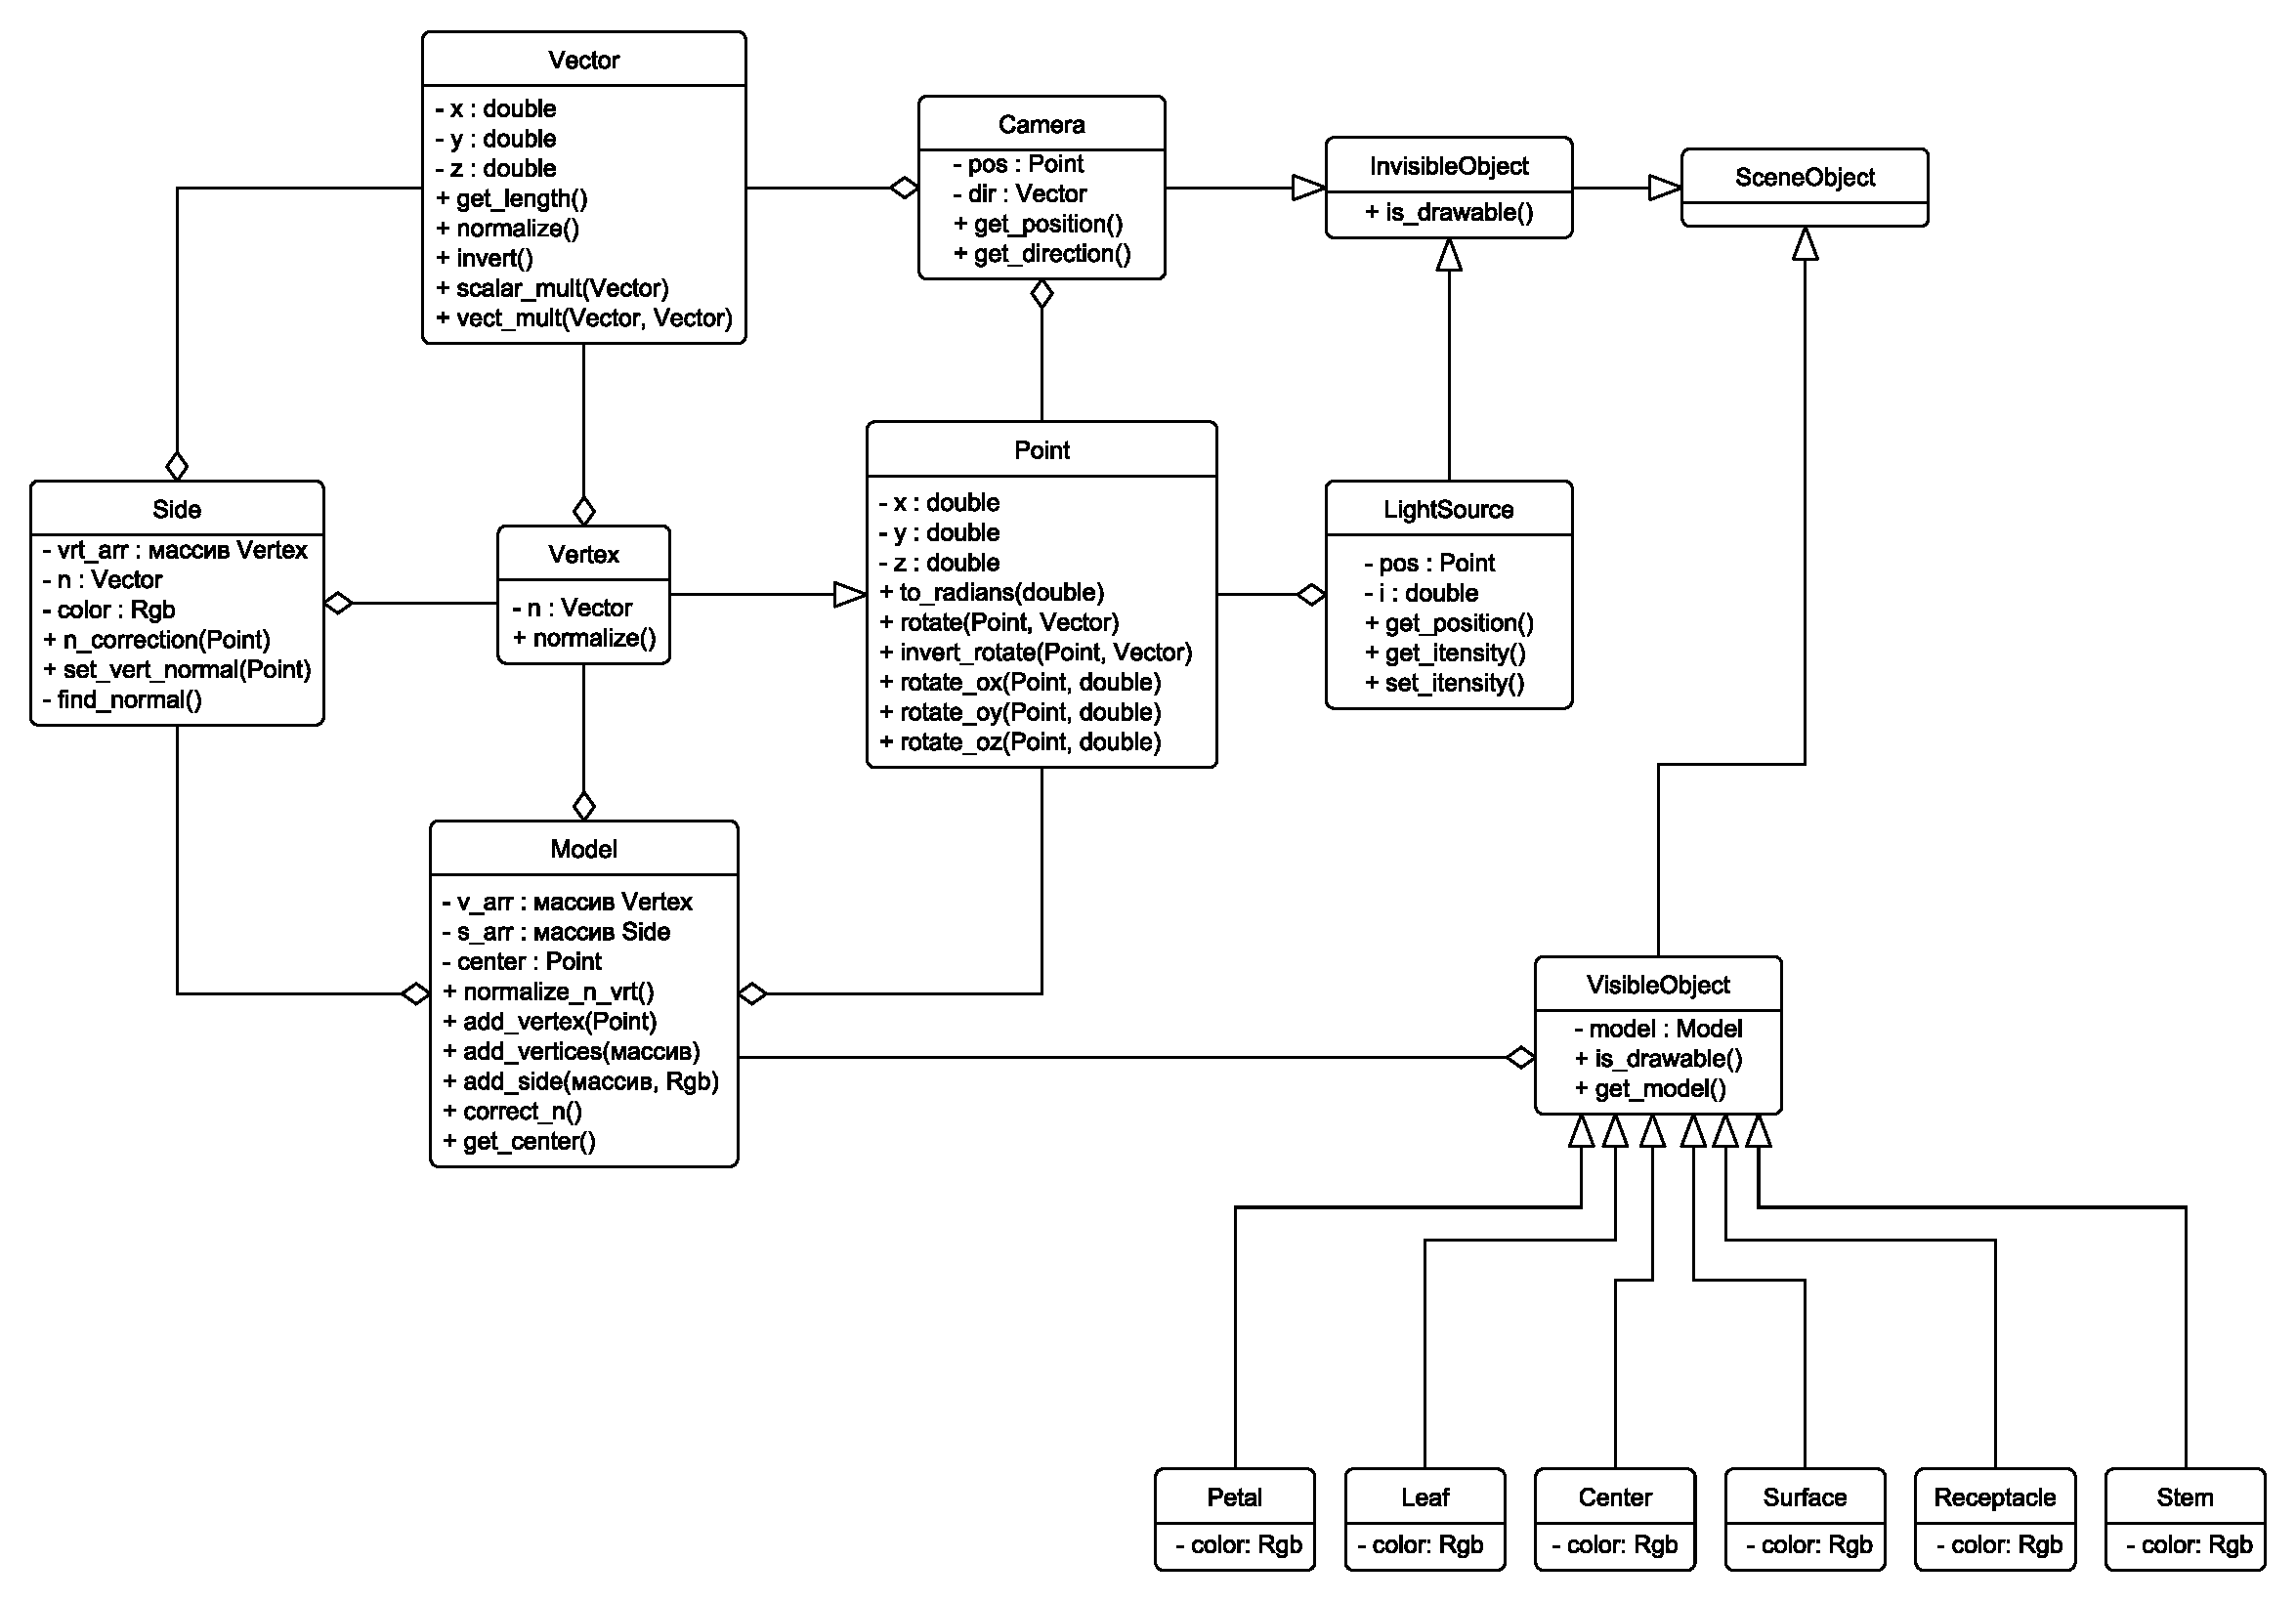
\includegraphics[angle=90,width=0.9\textwidth]{inc/img/uml}}
		\caption{Схема взаимодействия основных объектов сцены}
		\label{img:uml}
	\end{figure}

	
	\chapter{}
	Ниже приведены реализации классов основных объектов сцены.
	
	\lstinputlisting[frame=single, numbers=left, basicstyle=\footnotesize\ttfamily, title={Рисунок Б.1 -- Реализация класса точки}]{inc/lst/point.h}
	
	\lstinputlisting[frame=single, numbers=left, basicstyle=\footnotesize\ttfamily, title={Рисунок Б.2 -- Реализация класса вектора}]{inc/lst/vector.h}
	
	\lstinputlisting[frame=single, numbers=left, basicstyle=\footnotesize\ttfamily, title={Рисунок Б.3 -- Реализация класса вершины}]{inc/lst/vertex.h}

	\lstinputlisting[frame=single, numbers=left, basicstyle=\footnotesize\ttfamily, title={Рисунок Б.4 -- Реализация класса стороны}]{inc/lst/side.h}

	\lstinputlisting[frame=single, numbers=left, basicstyle=\footnotesize\ttfamily, title={Рисунок Б.5 -- Реализация класса камеры}]{inc/lst/camera.h}

	\lstinputlisting[frame=single, numbers=left, basicstyle=\footnotesize\ttfamily, title={Рисунок Б.6 -- Реализация класса источника света}]{inc/lst/lightsource.h}

	\lstinputlisting[frame=single, numbers=left, basicstyle=\footnotesize\ttfamily, title={Рисунок Б.7 -- Реализация класса модели}]{inc/lst/model.h}

	\lstinputlisting[frame=single, numbers=left, basicstyle=\footnotesize\ttfamily, title={Рисунок Б.8 -- Реализация класса лепестка}]{inc/lst/petal.h}

	\lstinputlisting[frame=single, numbers=left, basicstyle=\footnotesize\ttfamily, title={Рисунок Б.9 -- Реализация класса листа}]{inc/lst/leaf.h}
	
	\lstinputlisting[frame=single, numbers=left, basicstyle=\footnotesize\ttfamily, title={Рисунок Б.10 -- Реализация класса центральной части}]{inc/lst/center.h}
	
	\lstinputlisting[frame=single, numbers=left, basicstyle=\footnotesize\ttfamily, title={Рисунок Б.11 -- Реализация класса ограничивающей поверхности}]{inc/lst/surface.h}
	
	\lstinputlisting[frame=single, numbers=left, basicstyle=\footnotesize\ttfamily, title={Рисунок Б.12 -- Реализация класса цветоложа}]{inc/lst/receptacle.h}
	
	\lstinputlisting[frame=single, numbers=left, basicstyle=\footnotesize\ttfamily, title={Рисунок Б.13 -- Реализация класса стебля}]{inc/lst/stem.h}
	
	\chapter{}
	
	Ниже приведены реализации классов, отвечающих за визуализацию, трансформацию, смену времени суток.
	
	\lstinputlisting[frame=single, numbers=left, basicstyle=\footnotesize\ttfamily, title={Рисунок В.1 -- Реализация классов, отвечающих за визуализацию, трансформацию, смену времени суток}]{inc/lst/managers.h}
\end{appendices}

\end{document}